
%(BEGIN_QUESTION)
% Copyright 2010, Tony R. Kuphaldt, released under the Creative Commons Attribution License (v 1.0)
% This means you may do almost anything with this work of mine, so long as you give me proper credit

Flowdatamaskinen som er koblet til denne turbinstrømningsmåleren (med elektronisk pickup) registrerer ingen strømning, selv om vi vet at det faktisk går fluid gjennom røret. Et voltmeter koblet mellom terminalene TB1-1 og TB1-3 viser omtrent 11.0 volt DC og 10.8 volt AC ved en frekvens på 86 Hz:

$$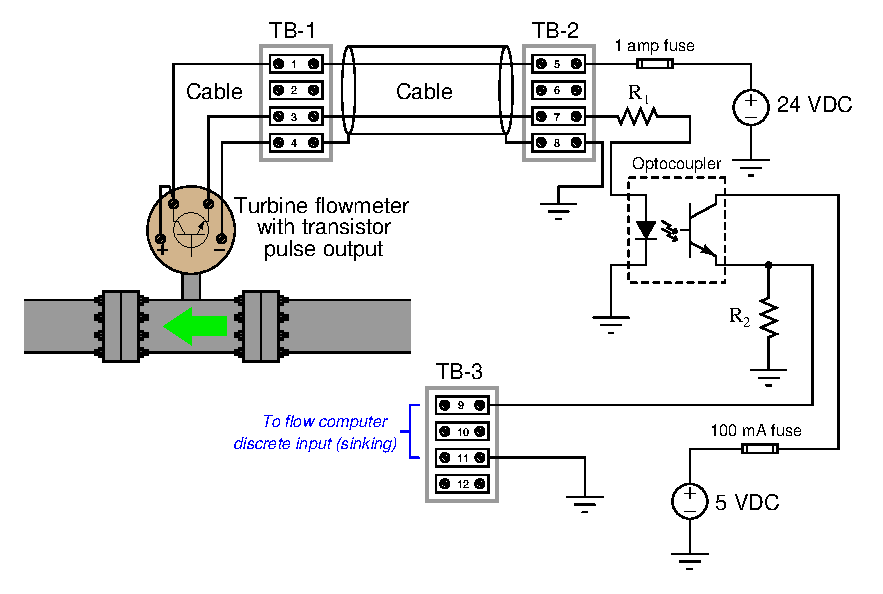
\includegraphics[width=15.5cm]{i00500x01.eps}$$

Bestem den diagnostiske verdien av hver av følgende tester. Anta at det bare finnes én feil i systemet, inkludert én enkelt komponent eller én enkelt leder/kabel/slange mellom komponenter. Hvis en foreslått test kan gi ny informasjon som hjelper deg å identifisere plasseringen og/eller arten til feilen, marker ``ja.'' Hvis testen ikke vil avsløre noe relevant for å identifisere feilen (som ikke allerede kan utledes av målingene og symptomene som er oppgitt), marker ``nei.''

% No blank lines allowed between lines of an \halign structure!
% I use comments (%) instead, so that TeX doesn't choke.

$$\vbox{\offinterlineskip
\halign{\strut
\vrule \quad\hfil # \ \hfil & 
\vrule \quad\hfil # \ \hfil & 
\vrule \quad\hfil # \ \hfil \vrule \cr
\noalign{\hrule}
%
% First row
{\bf Diagnostisk test} & {\bf Ja} & {\bf Nei} \cr
%
\noalign{\hrule}
%
% Another row
Mål DC-spenning mellom terminalene TB2-5 og TB2-8 &  &  \cr
%
\noalign{\hrule}
%
% Another row
Mål motstand mellom TB2-7 og TB2-8 med 1 A-sikringen trukket ut &  &  \cr
%
\noalign{\hrule}
%
% Another row
Mål DC-spenning over 100 mA-sikringen &  &  \cr
%
\noalign{\hrule}
%
% Another row
Mål DC-spenning over 1 A-sikringen &  &  \cr
%
\noalign{\hrule}
%
% Another row
Mål AC-spenning mellom terminalene TB3-9 og TB3-11 &  &  \cr
%
\noalign{\hrule}
%
% Another row
Mål kontinuitet i lederen mellom terminalene TB1-4 og TB2-8 &  &  \cr
%
\noalign{\hrule}
} % End of \halign 
}$$ % End of \vbox

\vfil 

\underbar{file i00500}
\eject
%(END_QUESTION)





%(BEGIN_ANSWER)

Dette er en vurdert oppgave -- ingen svar eller hint er gitt!

%(END_ANSWER)






%(BEGIN_NOTES)

Tilstedeværelsen av både DC- og AC-spenning ved pulssignalet fra strømningsmåleren forteller oss at vi har god kontinuitet mellom 24 VDC-kilden og transmitteren, og også at svitsjetransistoren faktisk pulserer av og på. Hvis den sto kontinuerlig på, ville vi bare målt noen få tidels volt DC. Hvis den sto kontinuerlig av, ville vi målt fulle 24 VDC hele tiden.

At voltmeteret viser en AC-spenning forteller oss at det ser en {\it oscillerende} spenning over tid. Dette betyr at transistoren faktisk svitsjer av og på slik den skal. I denne tilstanden, der signalet er en firkantbølge, vil voltmeteret vise en DC-spenning som er omtrent halvparten av DC-kildespenningen fordi det midler høy- og lavnivået i firkantbølgen. Ved 50\% duty cycle blir gjennomsnittlig DC-spenning 50\% av kildespenningen.

\vskip 10pt

Problemet ligger derfor enten i optokobleren eller videre nedstrøms (mot flowdatamaskinen). Tester som bare sjekker ledningsnett på strømningsmålerens krets (bortsett fra eventuelt diodekontroll i optokobleren) er derfor bortkastede tester.

% No blank lines allowed between lines of an \halign structure!
% I use comments (%) instead, so that TeX doesn't choke.

$$\vbox{\offinterlineskip
\halign{\strut
\vrule \quad\hfil # \ \hfil & 
\vrule \quad\hfil # \ \hfil & 
\vrule \quad\hfil # \ \hfil \vrule \cr
\noalign{\hrule}
%
% First row
{\bf Diagnostisk test} & {\bf Ja} & {\bf Nei} \cr
%
\noalign{\hrule}
%
% Another row
Mål DC-spenning mellom terminalene TB2-5 og TB2-8 &  & $\surd$ \cr
%
\noalign{\hrule}
%
% Another row
Mål motstand mellom TB2-7 og TB2-8 med 1 A-sikringen trukket ut &  & $\surd$ \cr
%
\noalign{\hrule}
%
% Another row
Mål DC-spenning over 100 mA-sikringen & $\surd$ &  \cr
%
\noalign{\hrule}
%
% Another row
Mål DC-spenning over 1 A-sikringen &  & $\surd$ \cr
%
\noalign{\hrule}
%
% Another row
Mål AC-spenning mellom terminalene TB3-9 og TB3-11 & $\surd$ &  \cr
%
\noalign{\hrule}
%
% Another row
Mål kontinuitet i lederen mellom terminalene TB1-4 og TB2-8 &  & $\surd$ \cr
%
\noalign{\hrule}
} % End of \halign 
}$$ % End of \vbox

\vfil \eject

\vskip 20pt \vbox{\hrule \hbox{\strut \vrule{} {\bf Virtuell feilsøking} \vrule} \hrule}

Denne oppgaven passer godt som en ``Virtuell feilsøking''-øvelse. Når du viser skjemaet til elevene, tenker du først ut en bestemt feil i systemet. Deretter presenterer du ett eller flere symptomer på denne feilen (noe en operatør eller bruker faktisk kan observere). Elevene foreslår så ulike diagnostiske tester for å finne feilens art og plassering, som om de var teknikere som feilsøkte anlegget. Din oppgave er å oppgi hvilke resultater hver foreslått test ville gitt, og dokumentere resultatene slik at alle elevene kan se dem.

Under og etter øvelsen er det nyttig å stille oppfølgingsspørsmål som:

\begin{itemize}
\item{} Hva forteller resultatet av den siste diagnostiske testen om feilen?
\item{} Anta at resultatet av den siste testen hadde vært annerledes. Hva ville det i så fall fortalt om feilen?
\item{} Er den siste testen den beste testen vi kunne gjort?
\item{} Hva ville vært den ideelle rekkefølgen på testene for å diagnostisere problemet i færrest mulig steg?
\end{itemize}


%INDEX% Troubleshooting review: electric circuit diagnostic test usefulness

%(END_NOTES)

